\begin{enumerate}
	\item Following the discussion of Example \ref{gp1}, interpret what it means for the associated graph of a relation $R$ if $R$ is 
	\begin{itemize}
		\item reflexive.
		\item symmetric.
	\end{itemize}
	\item Suppose Ryan presents you with the following graph associated with a relation $R$. He is very sad because the graph pictured is neither symmetric nor transitive. Add in the minimum number of necessary edges to make the relation\ldots
	\begin{itemize}
		\item reflexive.
		\item symmetric.
		\item transitive.
	\end{itemize}
\end{enumerate}
\begin{figure}[ht]
	\centering
	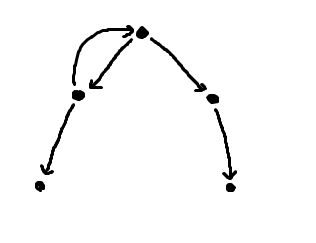
\includegraphics{Ch3/rgraph_ex1.png}
\end{figure}